\documentclass[main.tex]{subfiles}
\begin{document}
    \chapter{Embedded} 
    \label{ch:embedded}
    \section{Terminology}
Embedded-systems - AVR hardware programmed with custom in-house software stack, connected to sensors, and communicating with other devices through CAN and I$^2$C.\\
Control-Panel - UI interface running on a remote machine to visualize data and control pod \\
Master Machine - RaspberryPi 3B computer running Waterloop's communication-system software \\
Control/Sensor Hub - Arduino microcontroller running Waterloop's embedded-system software\\
CAN Data Packet - Custom communication packet type over CAN-BUS \\
Sensor Hub - centralized node for a group of sensors \\
Control Hub - centralized node for a group of control devices \\
HiL - Hardware in the Loop testing. Read more \href{https://en.wikipedia.org/wiki/Hardware-in-the-loop_simulation}{here} \\
WHiL - Waterloop's Hardware in the Loop testing software \\

      \begin{figure}
        \centering
        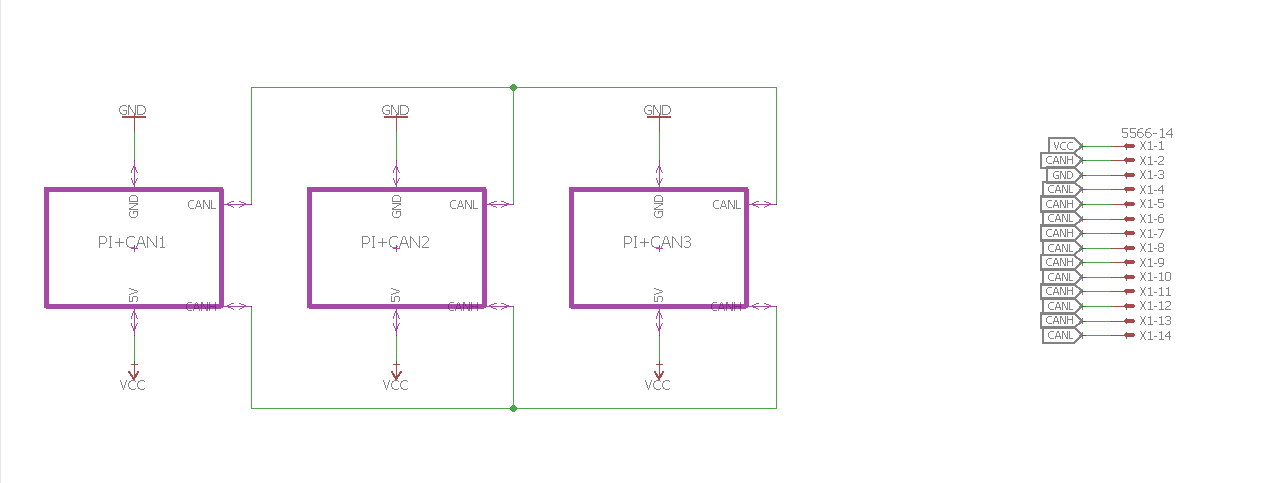
\includegraphics[width=\textwidth]{images/meb-rpi-mount.png}
        \caption{MEB RPIs circuit. Three RPIs are connected in parallel to the main pod CAN-BUS network, which is further extended to other devices on board.}
        \label{fig:meb-rpi-mount}
    \end{figure}
    
      \begin{figure}
        \centering
        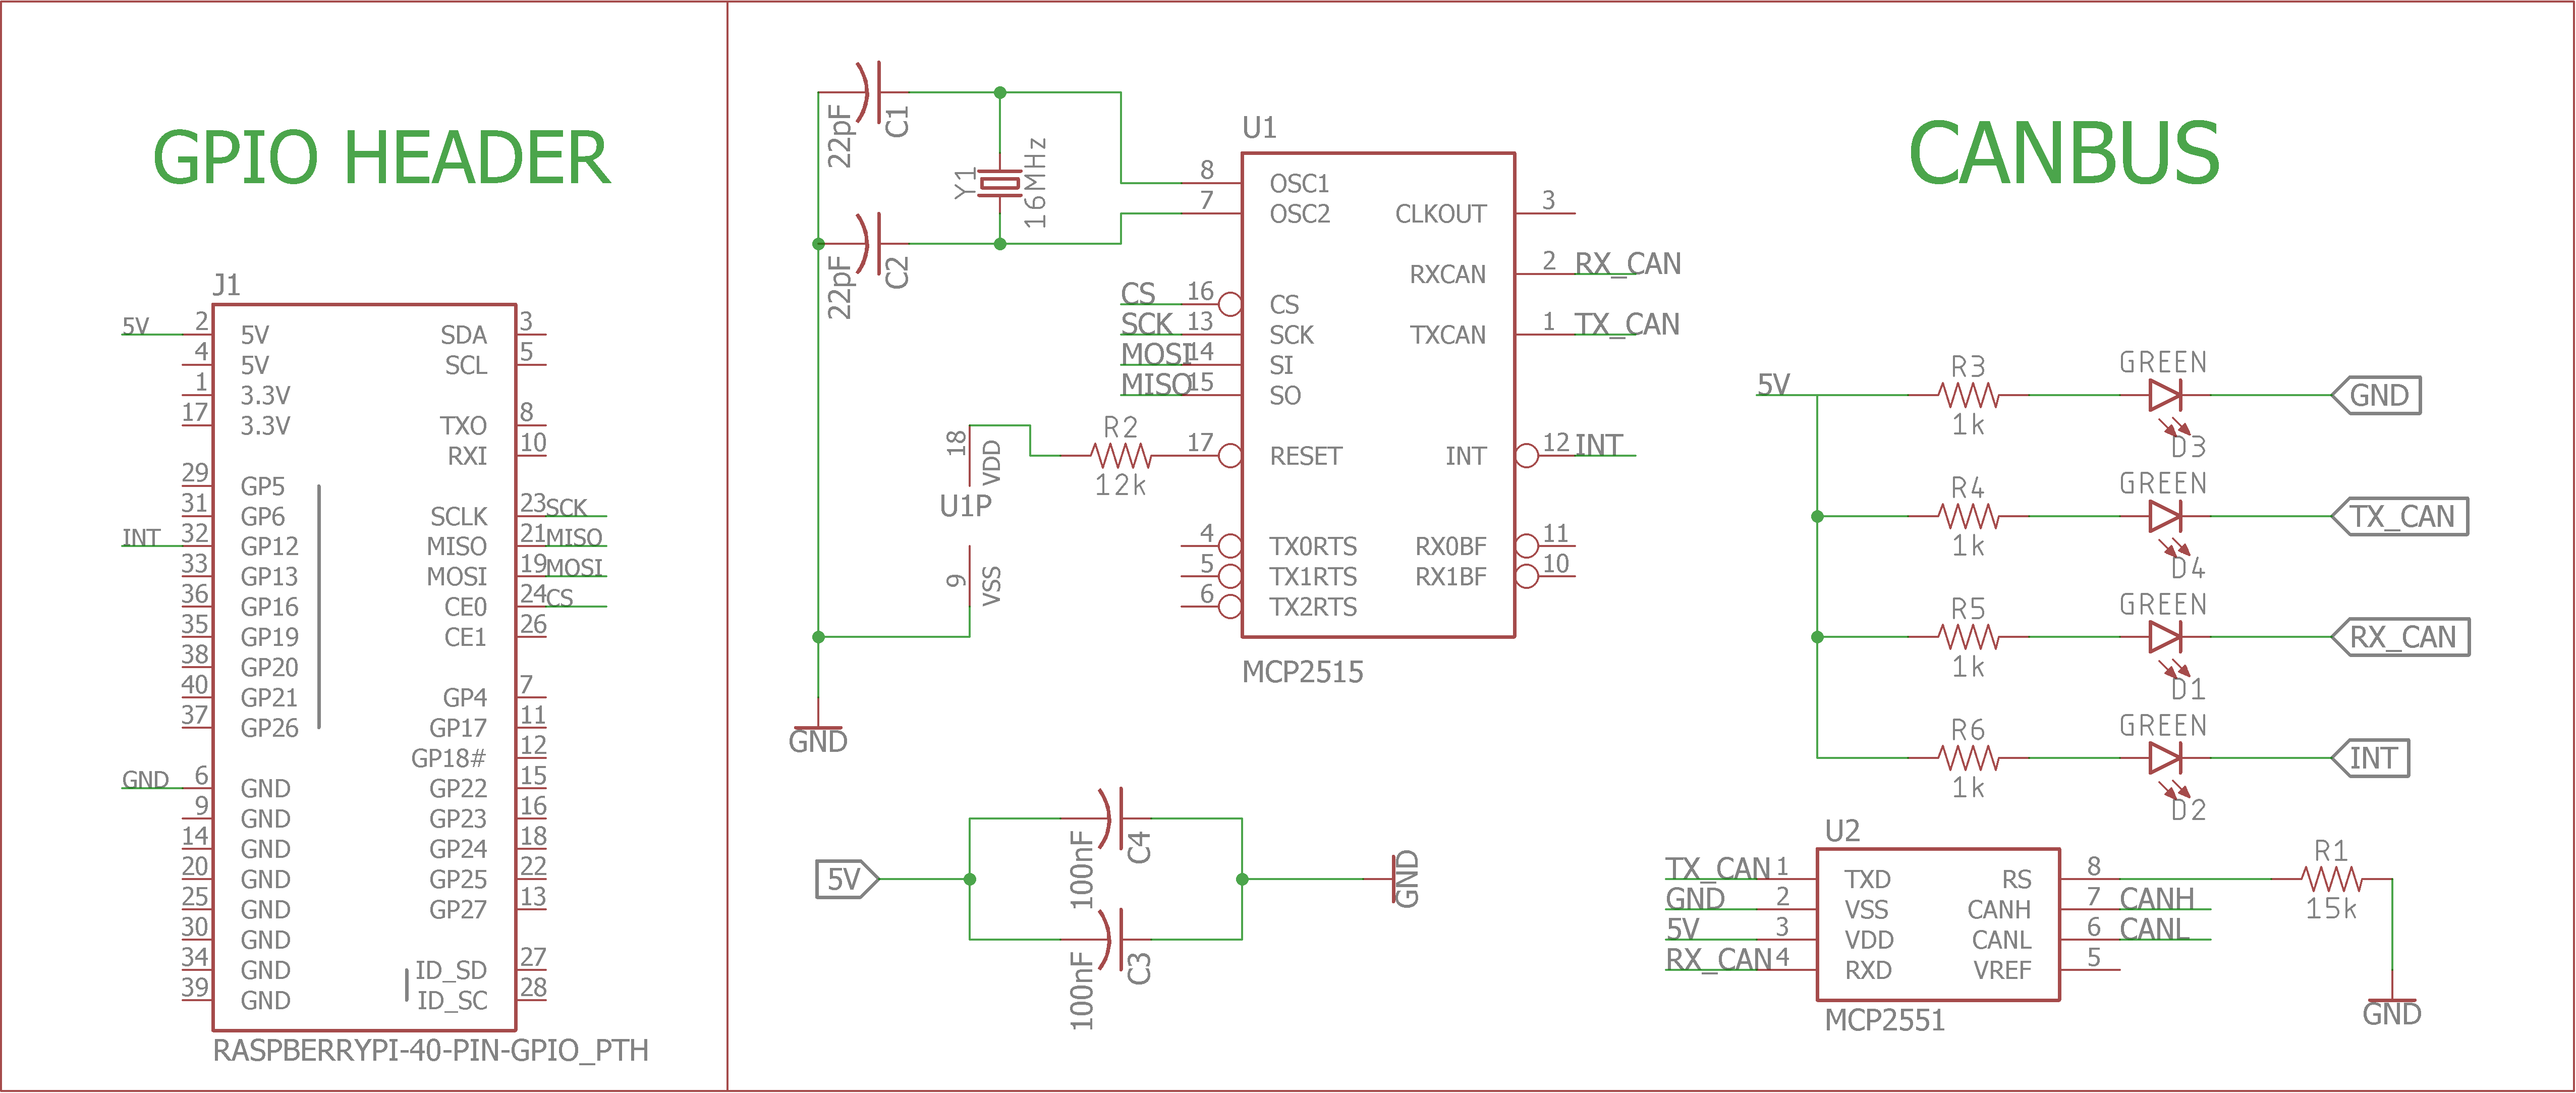
\includegraphics[width=\textwidth]{images/MEB_Module.png}
        \caption{One of the three Pi+CAN Modules. A raspberry Pi will be mounted on the board, and connected via ribbon cable to GPIO pins.}
        \label{fig:meb-module}
    \end{figure}

    \section{Main Embedded Board (MEB)}
    The Main Embedded Board (MEB) is the central hub for the Master Machines. For modularity and simplicity, the Raspberry Pis (RPis) are not integrated directly onto the MEB. Instead, three RPis are mounted (as described \reffig{fig:meb-rpi-mount}) onto the MEB (with insulation underneath the RPi. From there a board to board ribbon cable will be connected from the RPi to the MEB. Intergrated onto the MEB will be the MCP2515 and MCP2551 IC's which will allow the RPis to connect to the CAN-BUS network. External I/O on the MEB will include all the CANH and CANL lines from the Hub Processing Boards (which are explained in depth below), as well as 5V power. The design of modular RPis was chosen due to the fact that a board will 3 RPis being integrated into a singular board would have been cost, resource, and manpower inefficient
blown chip would have resulted in a waste of said resources. Thus it was decided to be more efficient to simply mount a OTS RPi onto the PCB as described above.


    \section{Hub Processing Boards (HPB)}
   	Hubs will be running embedded-systems software and will act as a data centralization point. Data collected from a series of grouped sensors will pass through an assigned Hub and will get packaged into CAN Data Packets for transmission to the Master Machines \textbf{See appendix blah-blah for details}.\\

\begin{table}
\begin{tabulary}{\textwidth}{@{}LLLLLL@{}} \toprule
	& Arduino Mega & Arduino Uno Rev3 & Arduino Due & Raspberry Pi 3B & Arduino Nano \\ \midrule
	Processor & ATmega2560 & ATmega328P & AT91SAM3X8E & 4 ARM Cortex-A53 & ATmega328P \\
    Clock Speed & 16 MHz & 16 MHz & 84 MHz & 1.2 GHz & 16MHz \\
    Operating Voltage & 5V & 3.3V & 3.3V & 5V & 5V \\
    \makecell[l]{Max. Operating\\Temperature} & 85 C & 85 C & 85 C & 85 C & 85 C \\
    GPIO & 54* & 14* 		& 54* & 26* & 30* \\
    Flash Memory & \SI{256}{KB}** & \SI{32}{KB}*** & \SI{512}{KB} & Varies & \SI{32}{KB} \\ \bottomrule
\end{tabulary}
\begin{flalign*}
  *&\quad\textrm{Expandable by third party shield}&\\
 **&\quad\textrm{\SI{8}{KB} of which is used by the bootloader}&\\
***&\quad\textrm{\SI{0.5}{KB} of which is used by the bootloader}&
\end{flalign*}
\caption{Hub Board Comparison}
\label{table:hub-board-comp}
\end{table}
After a comparison of different embedded boards (see \reftab{table:hub-board-comp}), Arduino Mega (ATmega) was selected as the preferred board due to its relatively high flash memory for AVR architecture. Although Arduino Due boasts better performance, our software systems does not have the need for the extra processing power and can function flawlessly on the ATmega2560 CPU. Each ATmega will be equipped with a CAN-BUS shield (built in-house), and each Hub will be running selectively compiled version of Embedded-systems to allow for a modular implementation of subsystem design. In order to allow for the use of packet priority on CAN-BUS network and further modularize the design, Hubs will be of two types: (1) Control Hubs and (2) Sensor Hubs.


  \begin{figure}
        \centering
        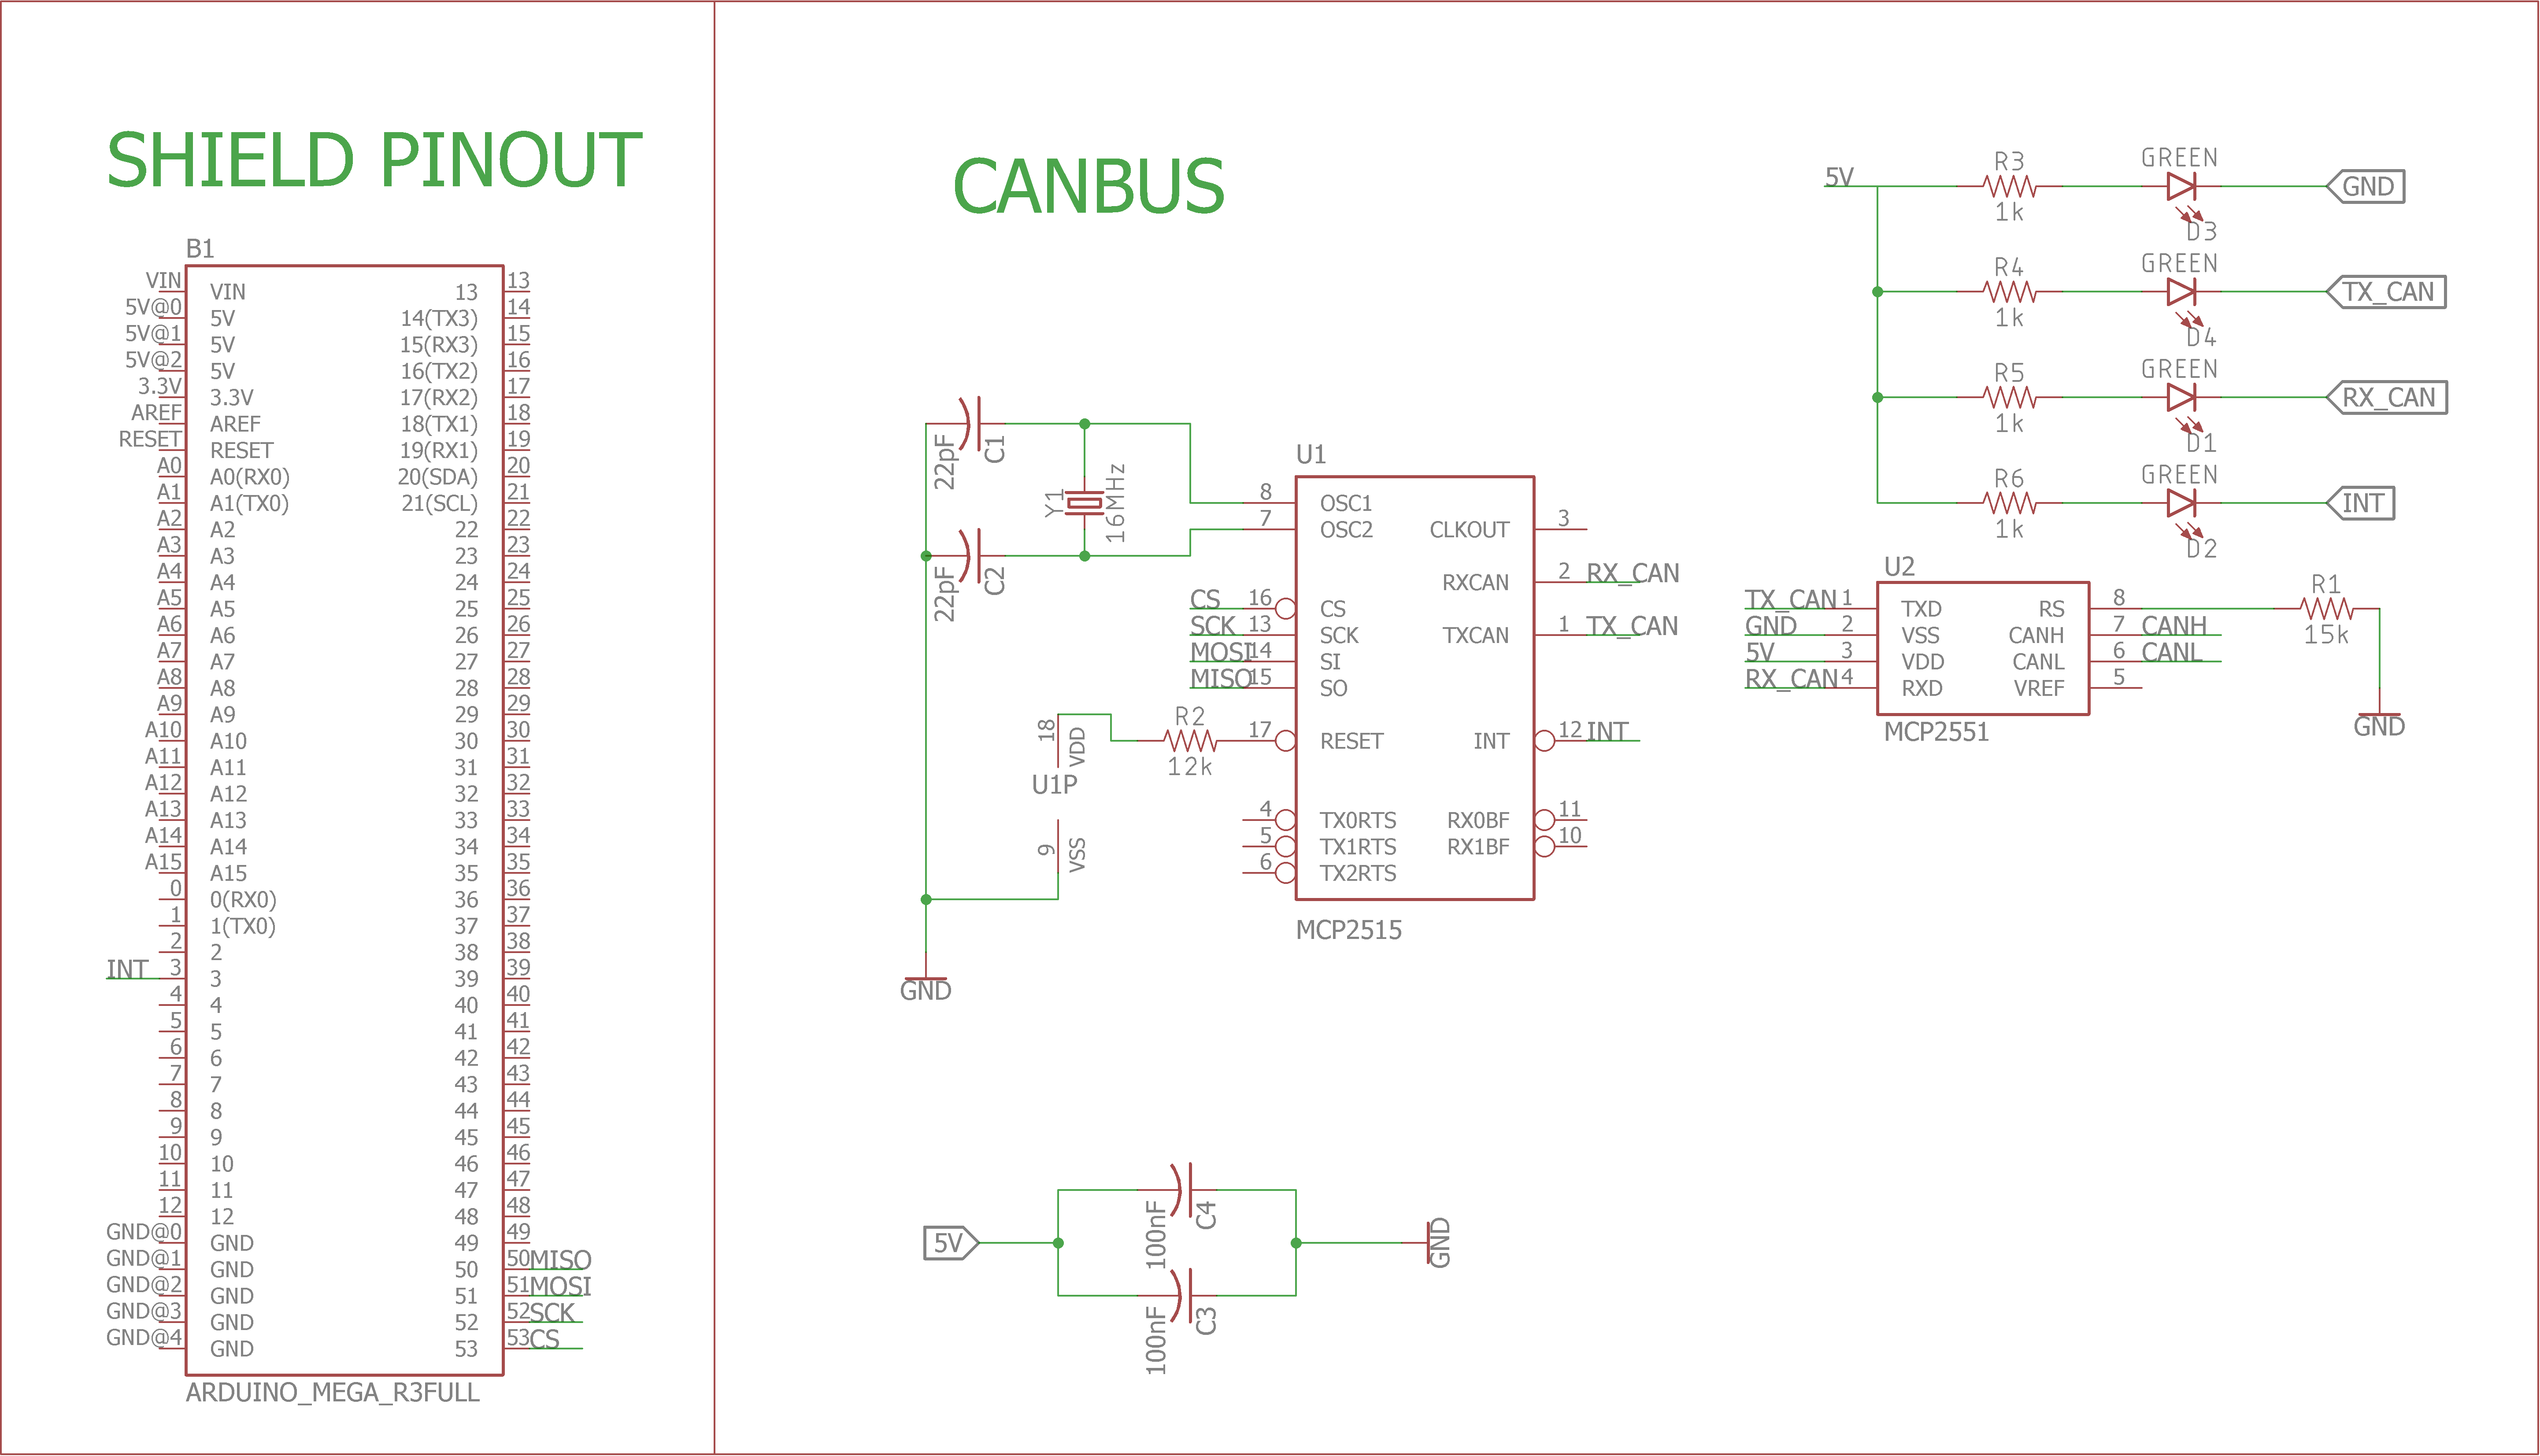
\includegraphics[width=\textwidth]{images/MEGA_SHIELD.png}
        \caption{Template schematic of Shield for Arduino Mega Module without I/O headers. Headers \& header connections to Mega will vary.}
        \label{fig:CAN Sheild}
    \end{figure}
    
    

\section{Sensor and Control Hubs}
\label{sec:sensor-and-control-hubs}
To make electrical debugging  easier and for efficient cable management, sensors on the pod will be distributed between multiple hubs on the pod. Specifically, three sensors hubs will be installed in the front, center, and rear of the pod, while the main control hub will be located at the center of the pod. Below is a detailed description of all Hub hardware and sensors/control elements

\begin{itemize}
	\item Sensor Hubs
    \begin{itemize}
    	\item Front Sensor Hub
        	\begin{itemize}
        		\item IMU Accelerometer
                \item Friction Brakes temperature
                \item Front-Wheel temperature
                \item Photoelectric Distance sensors x2
                \item MEMS-based 360 Tilt sensor
                \item Front friction piston solenoid temperature
        	\end{itemize}
        \item Central Sensor Hub
        	\begin{itemize}
            	\item IMU Accelerometer
                \item Liquid Cooling pressure
                \item 24V Battery current
        		\item EC-Brakes temperature x4
                \item Liquid Cooling temperature IN
                \item Liquid Cooling temperature OUT
                \item 24V Battery temperature
                \item EC-Brakes Solenoid temperature x2
                \item Main Battery temperature x4 
        	\end{itemize}
         \item Rear Sensor Hub
        	\begin{itemize}
                \item IMU Accelerometer
                \item Rear-Wheel temperature
        		\item Photoelectric Distance sensors x2
                \item Friction-drive motor temperature x2
                \item Rear friction piston solenoid temperature x2
                \item ESC temperature
        	\end{itemize}
    \end{itemize}
    \item Control Hub
    \begin{itemize}
    	\item Main control Hub
    	\begin{itemize}
        	\item Liquid Cooling
            \item Friction-Drive brakes
            \item EC-Brakes
            \item Rear friction solenoid x2
            \item Front friction solenoid x2
        \end{itemize}
    \end{itemize}
\end{itemize}

In addition to the Hub-Sensor distribution, \reftab{tab:pod-sensor-list} contains a list of sensors and all of the I/O pins required to wire electronic components.

\begin{table}
    \centering
    \begin{tabularx}{\linewidth}{@{}lccc@{}} \toprule
    Sensor & \makecell{\# of \\ Sensors} & \makecell{Description} & \makecell{Pins} \\ \midrule
    
    & & & \\
    \textbf{Temperature Sensors} & & & \\ \midrule
    Main Battery             & 4 & External, Contact      & GND, PW, ANALOG \\
    Motor                    & 2 & External, Contact      & GND, PW, ANALOG \\
    EC-Brake                 & 4 & External, Contactless  & SDA, SCL \\
    Embedded System          & 0 & Internal, CPU Built-in & GND, PW, ANALOG \\
    ESC                      & 1 & External, Contact      & GND, PW, ANALOG \\
    Liquid cooling (in/out)  & 2 & Internal, Threaded     & GND, PW, ANALOG \\
    Friction Drive Wheel     & 1 & External, Contactless  & SDA, SCL \\
    Friction Brakes          & 1 & External, Contactless  & SDA, SCL \\
    EC-solenoid              & 2 & External, Contactless  & SDA, SCL \\
    Friction Piston solenoid & 2 & External, Contactless  & SDA, SCL \\
    
    & & & \\
    \textbf{Current Sensors} & & & \\ \midrule
    Main Battery & 1 & Internal, BMS &\\
	24V Battery  & 1 & Internal, Built-In  &\\
    
    & & & \\
    \textbf{Tilt Sensors} & & & \\ \midrule
    Front Inclination Sensor & 1 & \makecell{MEMS-based \\ inclination sensors} & \makecell{PWR, GND, ANALOG x 2}\\
    
    & & & \\
	\textbf{Navigation Sensors} & & & \\ \midrule
    IMU Front & 1 & LSM6DS3 & \makecell{SDA, SCL, GND} \\
    IMU Centre & 1 & LSM6DS3 & \makecell{SDA, SCL, GND} \\
    IMU Back & 1 & LSM6DS3 & \makecell{SDA, SCL, GND}\\
    Shaft Encoder & 1 & Tamagawa TS2602N21E11 & GND, PW, ANALOG \\
    Electronic Speed Controller & 1 & UniTek Bamocar D3 & \makecell{+/-, M1, M2, M3, \\ CAN, I/O, RS232, Feedback}\\
    
	\textbf{Lateral Stability Sensors} & & & \\ \midrule
    \makecell{Photoelectric Distance Sensor \\ (2 at the front, 2 in the back)} & 4 &  & \makecell{PWR, (0-10V) Signal, \\ GND, GND (with resistor)} \\
    
    & & & \\
	\textbf{EC-Brakes Sensors} & & & \\ \midrule
    Reed Sensor & 2 & Basic REED switch & GND, DIGITAL \\
    
    & & & \\
    \textbf{Liquid Cooling Sensors} & & & \\ \midrule
    Pressure sensor & 2 & Internal, threaded & GND, PW, ANALOG, \\ Calibration, \\ Internal interface, Shield  \\\bottomrule
    \end{tabularx}
    \caption{Pod on-board sensor list. Total of 35 components that incorporate both control elements and necessary sensors.}
    \label{tab:pod-sensor-list}
\end{table}

\subsection{Sensors/Hubs Map}
As described in \refsec{sec:sensor-and-control-hubs}, all of the sensor and control data will be centralized and passed through Hubs on-board of the pod. With the importance of placement of electronic components on the pod, \reffig{fig:sensor-map} describes the mapping of all mounting locations.

  \begin{figure}
        \centering
        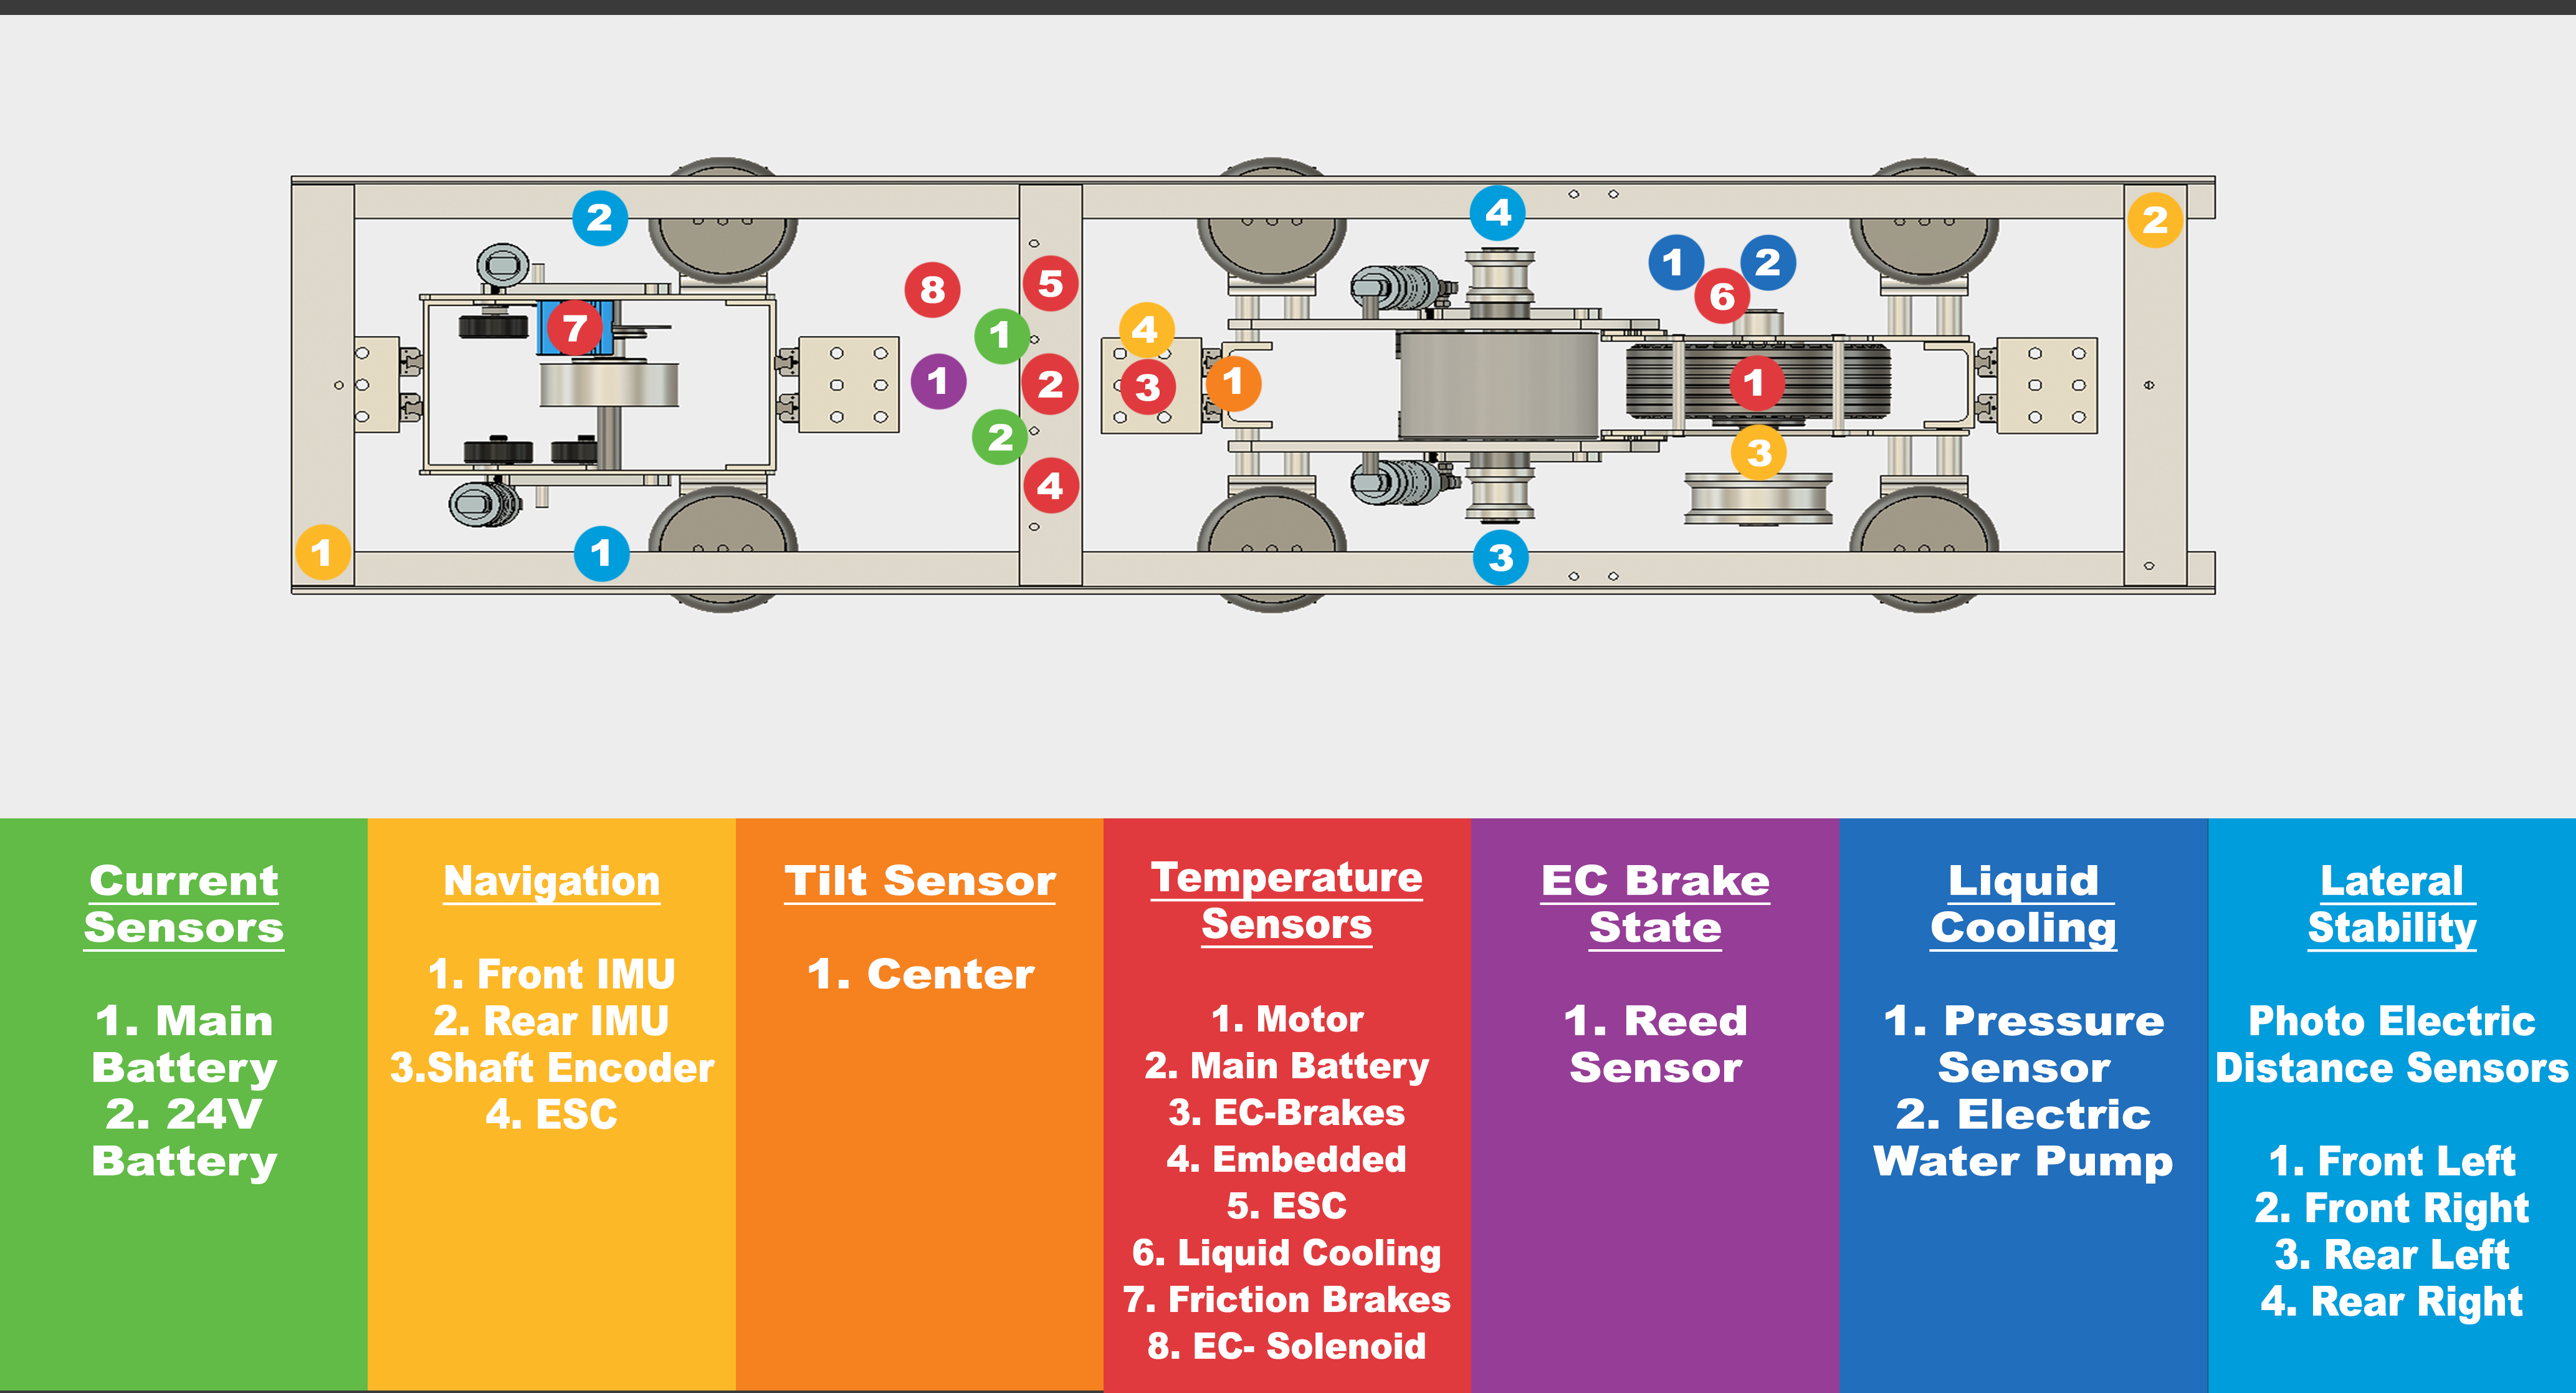
\includegraphics[width=\textwidth]{images/SENSOR.png}
        \caption{Goose 3 Sensor/Hub Map}
        \label{fig:sensor-map}
    \end{figure}

    \section{Library \& Build Infrastructure}
    To accommodate for unreliable nature of Arduino memory management libraries, Waterloop has developed a C++ library for use on AVR micro-controllers (Arduino and Raspberry Pi). While there are many alternatives available for memory management, libraries such as STL are overly complex which can result in unstable Arduino behavior. As a result, WLib is fast, memory efficient, has a small binary footprint, and is a safer alternative to STL. WLib uses a custom memory management solution with fixed-size memory blocks, preventing fragmentation and leaks. It provides basic data structures (lists, sets, maps, trees), and smart pointers (shared and unique). The library is open-sourced under MIT license and can be accessed though Waterloop's Github \url{https://teamwaterloop.github.io/waterloop-wlib/}

    Having no accessible building solutions that support Object Oriented Programing (OOP) for Arduino, Waterloop has also developed a custom Arduino build system with the use of Cosa. Cosa is an object-oriented AVR platform, that replaces standard Arduino libraries (\url{https://github.com/mikaelpatel/Cosa}) and provides faster performance and lower power consumption.
    
   \subsection{WLib}
   WLib is the library team Waterloop has specifically developed for the embedded-systems. Library has been created  to minimize the use of memory in Arduino systems which are naturally limited. \reffig{list:wlib-classes} shows a current list of the main components of the library.
   \begin{figure}
   \begin{multicols}{4}
        \begin{itemize}
            \item ArrayHeap
            \item ArrayList
            \item Bitset
            \item Comparator
            \item Hash
            \item HashMap
            \item HashSet
            \item HashTable
            \item HashSet
            \item LinkedList
            \item OpenMap
            \item OpenSet
            \item OpenTable
            \item Pair
            \item RedBlackTree
            \item SharedPtr
            \item Table
            \item TreeMap
            \item TreeSet
            \item Tuple
            \item TypeTraits
            \item UniquePtr
        \end{itemize}
        \end{multicols}
        \caption{WLib class list. A set of classes that is needed to support Embedded-systems software that will be running on HPBs. Additional sub-components have been developed as support elements to classes listed above}
	\label{list:wlib-classes}
\end{figure}
   
   \section{Hardware in the loop testing}
   \subsection{HiL testing description}
   Hardware in the Loop (HiL) simulation allows the entire domain of sensor inputs to be mapped to a particular state. For the purpose of the competition team Waterloop has developed it's own software to run HiL tests called WHiL. Based on the reading of the sensor, the state could return extreme ($y = 1, -1$) or acceptable ($y = 0$). This ensures that there is no ambiguity in the state of the pod at any moment. These states are expressed through piecewise functions, one of which is depicted on \reffig{fig:hil-function}:

  \begin{figure}
        \centering
        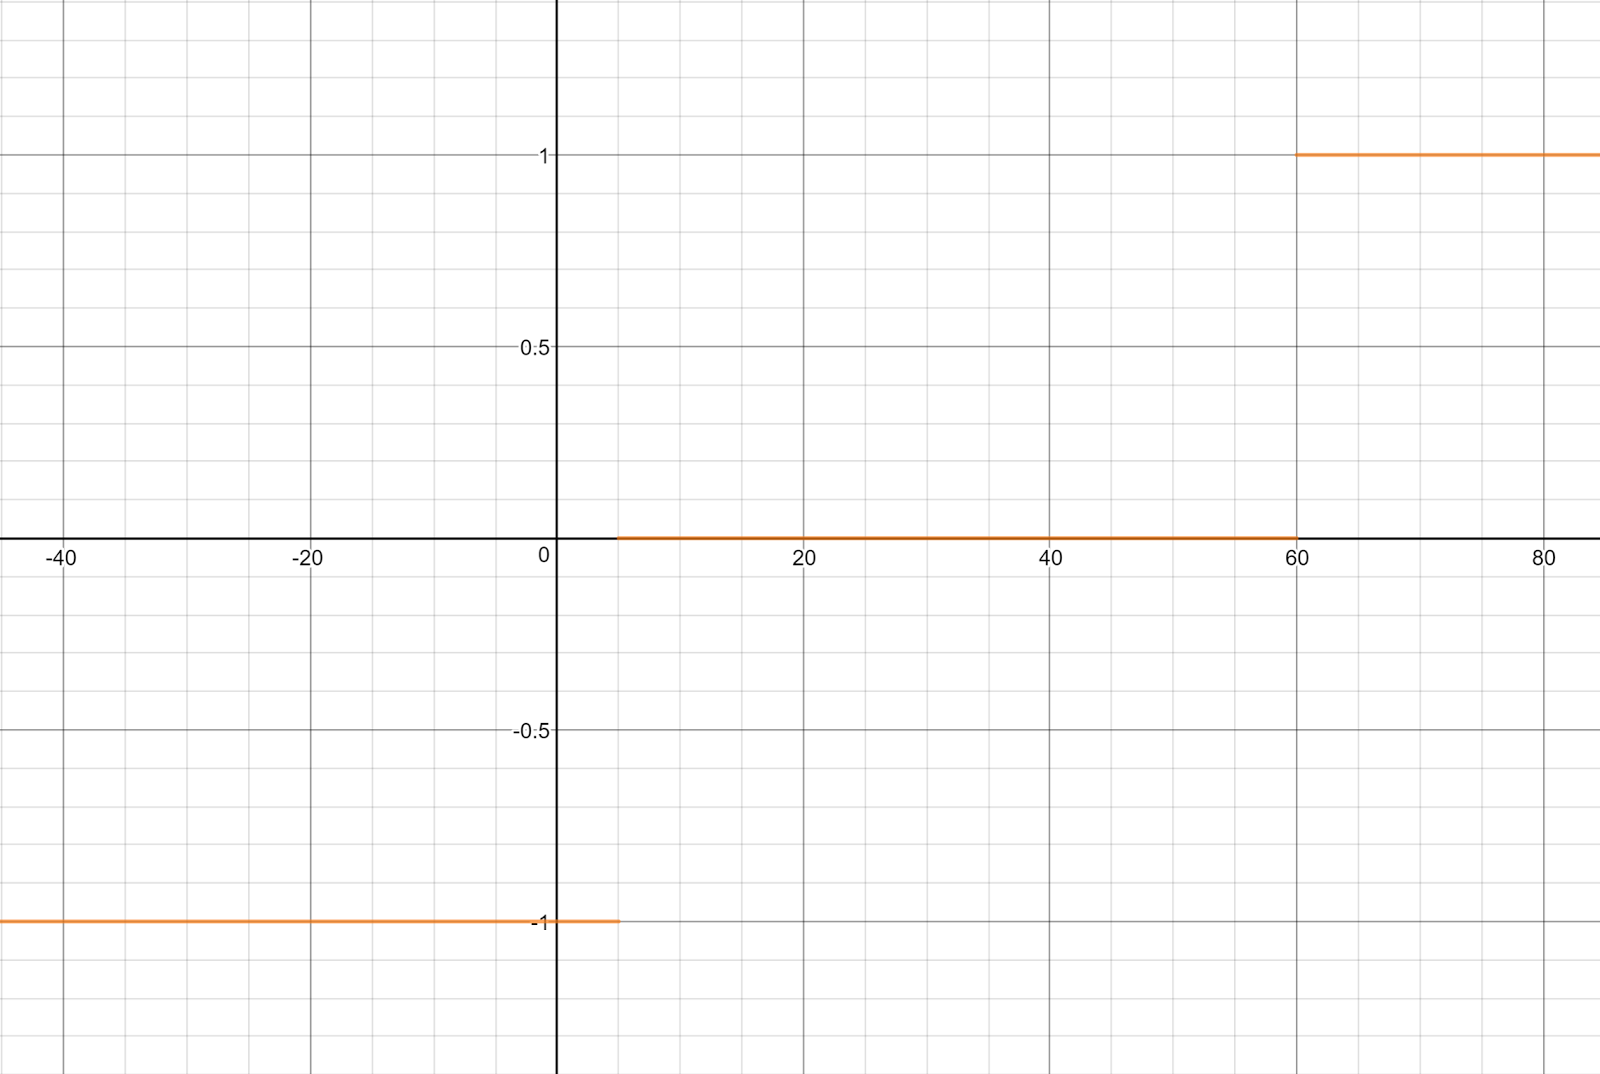
\includegraphics[width=\textwidth]{images/HiL-example-function.png}
        \caption{HiL example function. Domain: $(-\infty, \infty)$, Range: $\{-1,0,1\}$}
        \label{fig:hil-function}
    \end{figure}

\reffig{fig:hil-function} describes the function that refers to the battery temperature, friction drive temperature, brake temperature, and embedded system temperature.
Previous testing found that temperatures below 5 degrees or above 60 degrees Celsius constitute an extreme state for the pod, and are assigned non-zero values. This allows the state of the pod to be addressed in the context of critical and non-critical states. These values will be updated if needed during the build season.

\bigskip
\noindent Functions are given in the format 
	\begin{minted}{js}
    	y = {condition: "value", condition: "value", ...etc}
    \end{minted}
When the function returns $[1:-1]$ (with x as the sensor input value) there exists an extreme state. A full list of functions is given in \reftab{tab:hil-functions}.

\begin{table}
        \centering
        \begin{tabular}{@{}lc@{}} \toprule
        Sensors & Piecewise-defined Function \\ \midrule

        \makecell[l]{
          Battery temperature, friction drive \\ 
          temperature, brake temperature, \\ 
          embedded system temperature, \\
          IMU front and back temperature
        } & 
        \makecell{
          $y = \{ x > 60:1, x < 5:-1,5 \leq x \leq 60 : 0 \}$ \\
          x : temperature in degrees Celsius
        } \\ 

        \makecell[l]{
          Liquid cooling temperature, \\
          ESC temperature
        } & 
        \makecell{
          $y = \{ x > 105:1, x < -30:-1, -30 \leq x \leq 105:0 \}$ \\ 
          x : temperature in degrees Celsius
        } \\

        \makecell[l]{
          Main battery current
        } & 
        \makecell {
          $y = \{ x > 250:1, x < 5:-1, 250 \leq x \leq 5 :0 \} $ \\ 
          x : current in amperes
        } \\

        \makecell[l]{
          Inclination sensor
        } & 
        \makecell{
          $y = \{ x > 3: 1, x < -3 : -1, -3 \leq x \leq 3: 0 \}$ \\ 
          x : angle in degrees
        } \\

        \makecell[l]{
          IMU front and back magnetometer
        } & 
        \makecell{
          $y = \{ x > 800:1, x < 0:-1, 800 \leq x \leq 0:0 \}$ \\
          x: magnetic field strength in gauss
        } \\

        \makecell[l]{
          Photoelectric distance
        } & 
        \makecell{
          $y = \{ x > 20:1, x < 8:-1, 8 \leq x \leq 20:0 \}$ \\ 
          x: distance in millimeters
        } \\

        \bottomrule
        \end{tabular}
        \caption{HiL testing functions. Each sensor is described using a piecewise defined function, which allows to have test inputs on a continuous domain.}
        \label{tab:hil-functions}
    \end{table}

    \subsection{HiL testing setup}
    Desktop application has been created to easily test the embedded components of our system. Qt and C++ are the technologies Waterloop used to build an application that is capable of testing the different pins of an Arduino Mega boards with predefined inputs. The program transmits binary values to various digital pins and numerical values to analog pins.
   
    System is built by introducing three machines: (1) Input Machine. (2) Transmitter Machine, (3) Control Machine. \reffig{fig:hil-testing-rig} demonstrates the outline of the system.
   
      \begin{figure}
        \centering
 		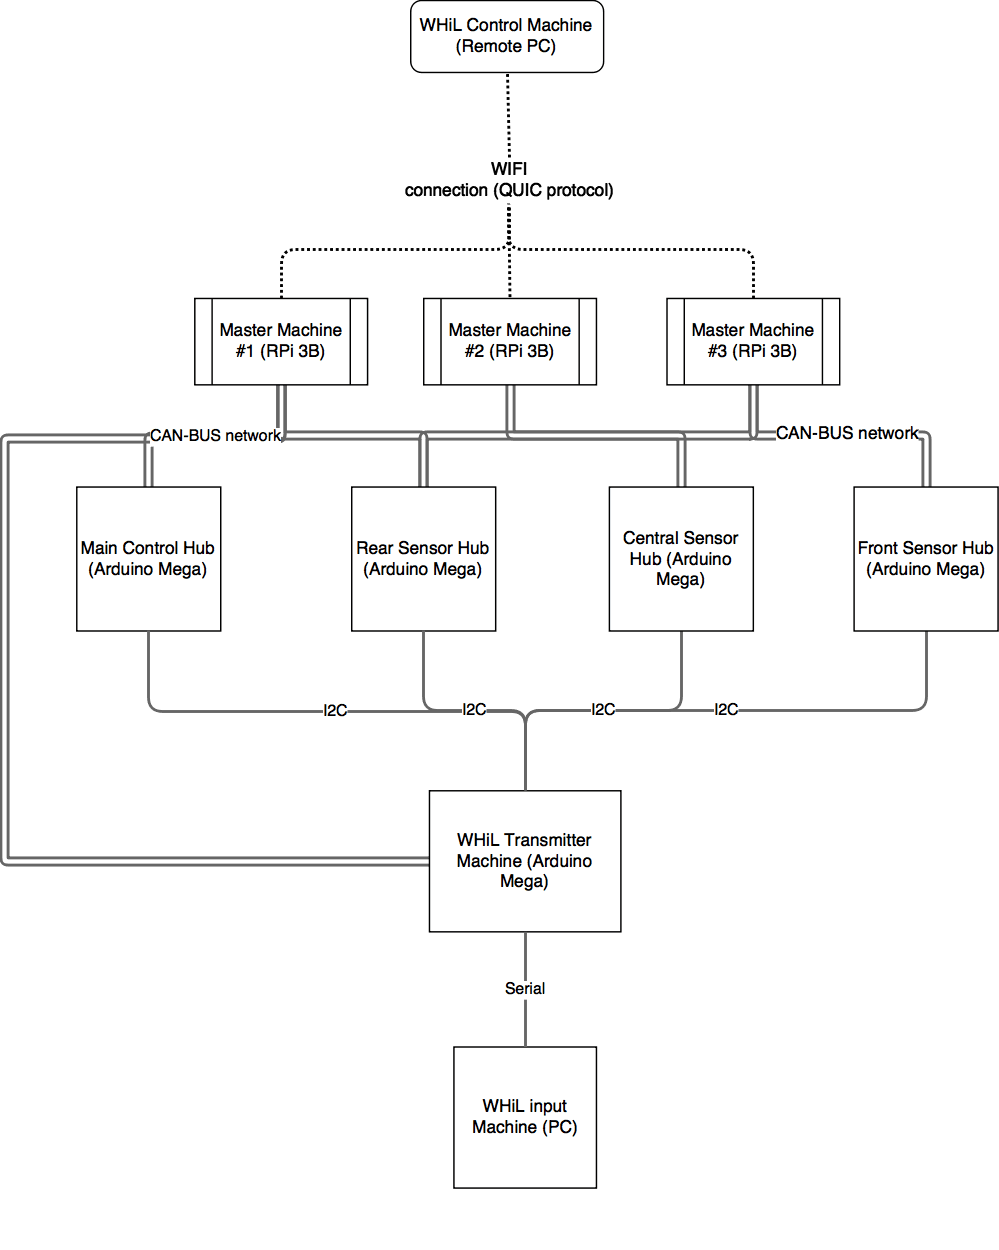
\includegraphics[width=\textwidth]{images/hil_testing_rig.png}
		\caption{WHiL testing rig outline. Data flows from Input machine into a Transmitter machine, which uses a combination of Analog, Digital and CAN-BUS communication pipelines to simulate pod launches and test the performance of on-board Embedded systems. After all the internal computation is complete by the Embedded-systems, Master Machines output the data to the Control Machines, which verifies it in place.}
        \label{fig:hil-testing-rig}
   \end{figure}
   
   WHiL Software works by generating a series of JSON files These objects are later sent to WHiL Transmitting machine through serial communication powered by QSerialPort\footnote{Qt Serial Library ``QSerialPort'' \url{http://doc.qt.io/qt-5/qserialport.html}}. The JSON objects received through serial communication are then converted to C++ objects using the ArduinoJson\footnote{ArduinoJson GitHub: \url{https://github.com/bblanchon/ArduinoJson}} open-source framework. These objects are then used to test the states and conditions of ATMegas or sent into the CAN-BUS network. \reffig{fig:hil-pin-selection} shows the pin selection interface developed for quick test creation and fast iteration process.
   
   \begin{figure}
        \centering
 		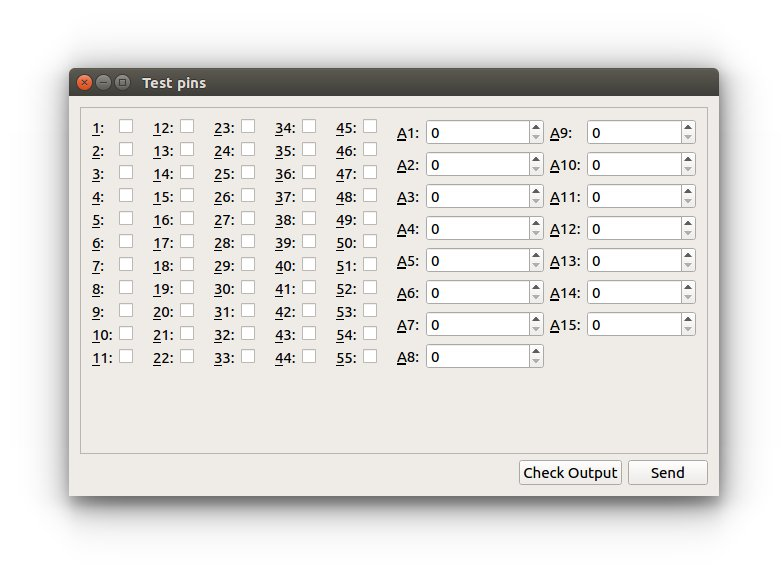
\includegraphics[width=\textwidth]{images/pin-testing.jpg}
		\caption{WHiL pin input selection interface. Having a GUI interface for test creation allows for much faster test iteration process}
        \label{fig:hil-pin-selection}
   \end{figure}
   
\section{Embedded Bill of Materials}
    \reftab{tab:emb-bom} provides a complete cost breakdown of all on-board sensors and control elements. Most of the components will be purchased online with a few being reused from previous competitions. Sourcing strategy for all elements has been already developed and orders will be placed mid-January to have components delivered as soon as possible.
    
\end{document}